\documentclass[11pt]{article}

\usepackage[banglamainfont=Kalpurush, banglattfont=Siyam Rupali, feature=0, changecounternumbering=0]{latexbangla}
\usepackage[top=8em, left=8em, right=8em, bottom=8em]{geometry}
\usepackage{verbatim,spverbatim, hyperref, tcolorbox, hologo, enumerate, amsthm, xpatch, amsfonts, amssymb, amsmath, enumerate, chngcntr, pgffor,dirtytalk}
\usepackage{tikz}
\usetikzlibrary{calc,trees,positioning,arrows,fit,shapes,calc}
\hypersetup{hidelinks=yes}
\tcbuselibrary{breakable}

\def\fileversion{v0.2}
\def\filedate{31 October, 2016}
\def\latexbangla{\hologo{LaTeX}\texttt{bangla}}
\newcommand{\pkn}[1]{\texttt{#1}}
\addto\captionsbengali{%
  \renewcommand{\contentsname}{Table of Contents}%
}

\makeatletter
%making the word "proof" in proof env. bold and adding a : after it.	
\xpatchcmd{\proof}{\itshape}{\bfseries}{}{}
\xpatchcmd{\proof}{\@addpunct{.}}{\@addpunct{:}}{}{}
\linespread{1.1}	
\def\@banglanumber#1{\expandafter\@@banglanumber\number#1\@nil}
\def\@@banglanumber#1{\ifx#1\@nil
\else\char\numexpr#1+"09E6\relax\expandafter\@@banglanumber\fi}
\def\tobangla#1{\expandafter\@banglanumber\csname c@#1\endcsname}
\def\numtobangla#1{\@@banglanumber#1\@nil}\addto\captionsbengali{\renewcommand\proofname{\bfseries প্রমাণ}}
\newenvironment{solution}{\proof[\bfseries সমাধান]}{\endproof}

\newtheoremstyle{custom}% name
{3pt}% space above
{3pt}% space below
{\rm}% body font
{}% indent amount
{\bfseries}% theorem head font
{:}% punctuation after theorem head
{.5em}% space after theorem head
{}% theorem head spec
\theoremstyle{custom}
\newtheorem{problem}{\bfseries সমস্যা}
\renewcommand{\theequation}{\thesection.\tobangla{equation}}
\renewcommand{\theproblem}{\tobangla{problem}}
\makeatother




\title{The \latexbangla~Package\\
Enhanced \LaTeX\ integration for Bangla}
\author{Adib Hasan\\
\texttt{adib.hasan8@gmail.com}}
\date{\filedate\qquad\fileversion}

\begin{document}
\maketitle
\tableofcontents
\pagebreak
\section{Definition}
Function is a special case of relation, from a non empty set $A$ to a non empty set $B$, that associates each member of $A$ to a unique member of $B$. Symbolically, we write $f: A \rightarrow B$. We read it as \say{$f$ is a function from $A$ to $B$}.
Set $A$ is called domain of f and set $B$ is called co-domain of $f$.
For example, let $A = \{–1, 0, 1\}$ and $B=\{0, 1, 2\}$. Then $A\times B = \{(–1, 0), (–1, 1), (–1, 2), (0, 0), (0, 1), (0, 2), (1, 0),(1, 1), (1, 2)\}$
Now, \say{$f: A \rightarrow B$ defined by $f(x) = x^2$} is the function such that $f = \{(–1, 1), (0, 0), (1, 1)\}$. $f$ can also be show diagramatically by following picture:

\begin{figure}[h]
 \centering
 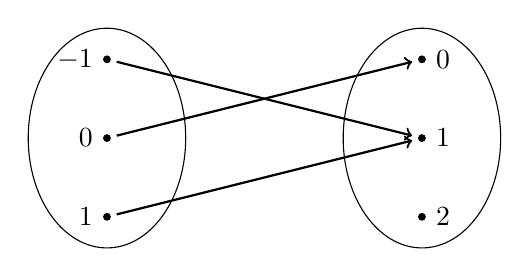
\begin{tikzpicture}[ele/.style={fill=black,circle,minimum width=.8pt,inner sep=1pt},every fit/.style={ellipse,draw,inner sep=-2pt}]
  \node[ele,label=left:$-1$] (a2) at (0,3) {};    
  \node[ele,label=left:$0$] (a3) at (0,2) {};
  \node[ele,label=left:$1$] (a4) at (0,1) {};

  \node[ele,,label=right:$0$] (b2) at (4,3) {};
  \node[ele,,label=right:$1$] (b3) at (4,2) {};
  \node[ele,,label=right:$2$] (b4) at (4,1) {};

  \node[draw,fit= (a2) (a3) (a4),minimum width=2cm] {} ;
  \node[draw,fit=  (b2) (b3) (b4),minimum width=2cm] {} ;  
  \draw[->,thick,shorten <=2pt,shorten >=2] (a2) -- (b3);
  \draw[->,thick,shorten <=2pt,shorten >=2] (a3) -- (b2);
  \draw[->,thick,shorten <=2pt,shorten >=2] (a4) -- (b3);
 \end{tikzpicture}
\end{figure}

Every function say $f : A \rightarrow B$ satisfies the following conditions:\\
(a) $f \subseteq A\times B$, (b) $\forall a\in A \Rightarrow (a, f(a)) \in f$ and (c) $(a, b)\in f\, \&\, (a, c) \in f \Rightarrow b = c$
\section{How to use}
\subsection{Sample Code}
Here is the simplest example for \latexbangla:
\begin{tcolorbox}[breakable]
\begin{verbatim}
\documentclass{article}
\usepackage[banglamainfont=Kalpurush, 
            banglattfont=Siyam Rupali
           ]{latexbangla}
\begin{document}
পিথাগোরাস(Pythagoras)-এর উপপাদ্যটি হল,\\
\textit{সমকোণী ত্রিভুজের অতিভুজের উপর অঙ্কিত বর্গক্ষেত্রের ক্ষেত্রফল অপর দুই বাহুর 
উপর অঙ্কিত বর্গক্ষেত্রের ক্ষেত্রফলের সমষ্টির সমান।}\\
অর্থাৎ কোন সমকোণী ত্রিভুজের অতিভুজ $c$ এবং অপর দুই বাহু $a$ এবং $b$ হলে,
\[c^2=a^2+b^2\]
লক্ষ্য করুন, এখন পর্যন্ত টেক্সট প্রদর্শনের জন্য \textbf{কালপুরুষ} ফন্ট ব্যবহৃত হয়েছে।\\
\texttt{এবার, টেলিটাইপ(Teletype) টেক্সট প্রদর্শনের জন্য \textbf{সিয়াম রূপালী} 
ফন্ট ব্যবহৃত হল।}\\
পুনরায় টেক্সট প্রদর্শনের জন্য \textbf{কালপুরুষ} ফন্ট ব্যবহৃত হচ্ছে।
\end{document}
\end{verbatim}
\end{tcolorbox}
\begin{tcolorbox}[breakable, colback=white]
পিথাগোরাস(Pythagoras)-এর উপপাদ্যটি হল,\\
\textit{সমকোণী ত্রিভুজের অতিভুজের উপর অঙ্কিত বর্গক্ষেত্রের ক্ষেত্রফল অপর দুই বাহুর 
উপর অঙ্কিত বর্গক্ষেত্রের ক্ষেত্রফলের সমষ্টির সমান।}\\
অর্থাৎ কোন সমকোণী ত্রিভুজের অতিভুজ $c$ এবং অপর দুই বাহু $a$ এবং $b$ হলে,
\[c^2=a^2+b^2\]
লক্ষ্য করুন, এখন পর্যন্ত টেক্সট প্রদর্শনের জন্য \textbf{কালপুরুষ} ফন্ট ব্যবহৃত হয়েছে।\\
\texttt{এবার, টেলিটাইপ(Teletype) টেক্সট প্রদর্শনের জন্য \textbf{সিয়াম রূপালী} 
ফন্ট ব্যবহৃত হল।}\\
পুনরায় টেক্সট প্রদর্শনের জন্য \textbf{কালপুরুষ} ফন্ট ব্যবহৃত হচ্ছে।
\end{tcolorbox}
As you see, no special command was required to switch language or to use any other facility. With \latexbangla, you don't need to learn a hundred new commands to type Bangla. You simply type normal \hologo{LaTeX} syntax and expect everything to work as it should. 

\latexbangla~does have some limitations, however. (Most of which are due to my lack of time to implement solutions.) So, do take a look at the known issues section.
\section{Functionalities}
\subsection{Package options}
Package options are listed below:\vspace*{2mm}
\begin{itemize}
\renewcommand\labelitemi{}

\item\noindent\texttt{banglamainfont}\textbf{(Required)}\\
Sets the default Bangla font for the document, but does not affect the Latin characters. (They are rendered by the \hologo{LaTeX} default Latin Modern font.) \latexbangla~will automatically fake bold, italic and bolditalic variants for \pkn{banglamainfont} if no font from the appropriate subfamily is found.\\

\item\texttt{banglattfont}\textbf{(Required)}\\
The default Teletype Bangla font. (Again, Latin characters are rendered by the \hologo{LaTeX} default Latin Modern Teletype.) \latexbangla~will also fake bold, italic and bolditalic variants automatically for this font if no font from the appropriate subfamily is found.\\

\item\texttt{feature}(Optional, default=1)(\texttt{0->none, 1->recommended, 2->full})\\
To which extent \latexbangla~should enable additional features. For \pkn{feature=1}, the following features will be enabled:
\begin{enumerate}
\item the following packages are loaded: \pkn{titlesec, amsthm, xpatch, amsfonts, amssymb, amsmath, enumerate, chngcntr}.
\item a ``Dot" is added after chapter, section, subsection etc. numbers.
\item \textit{প্রমাণ.} is replaced by \textbf{প্রমাণ:} in \pkn{proof} environment.
\item Line height is set to 110\%.
\item A new command \verb|\tobangla{counter name}| is defined. (See commands subsection for description)
\item \pkn{example, problem, solution, theorem} environments are defined. The counter associated with \texttt{theorem} environment resets in every section.
\item The counters associated with \pkn{enumerate, footnote} environments are converted to Bangla.
\end{enumerate}
\begin{tcolorbox}[breakable]
\begin{verbatim}
\usepackage[banglamainfont=Kalpurush,
            banglattfont=Siyam Rupali,
            ]{latexbangla}
\begin{document}
\begin{problem}
$p$ একটি মৌলিক সংখ্যা এবং $n$ একটি স্বাভাবিক সংখ্যা হলে প্রমাণ কর যে 
$p|n^p-n$ 
\end{problem}
\begin{proof}
$p|n$ হলে এটি স্বাভাবিকভাবেই সত্যি। অন্যথায়, $\{n,2n,\ldots,(p-1)n\}$
 একটি পূর্ণাঙ্গ রেসিডিও ক্লাস তৈরি করে। যার ফলে...
\end{proof}
\begin{problem}
$a$ এবং $n$ পরস্পর সহমৌলিক স্বাভাবিক সংখ্যা হলে দেখাও যে $a^{\phi(n)}
\equiv 1\pmod n$
\end{problem}
\end{document}
\end{verbatim}
\end{tcolorbox}
\begin{tcolorbox}[breakable, colback=white]
\begin{problem}
$p$ একটি মৌলিক সংখ্যা এবং $n$ একটি স্বাভাবিক সংখ্যা হলে প্রমাণ কর যে $p|n^p-n$ 
\end{problem}
\begin{proof}
$p|n$ হলে এটি স্বাভাবিকভাবেই সত্যি। অন্যথায়, $\{n,2n,\ldots,(p-1)n\}$ একটি
পূর্ণাঙ্গ রেসিডিও ক্লাস তৈরি করে। যার ফলে...
\end{proof}
\begin{problem}
$a$ এবং $n$ পরস্পর সহমৌলিক স্বাভাবিক সংখ্যা হলে দেখাও যে $a^{\phi(n)}\equiv 1\pmod n$
\end{problem}
\end{tcolorbox}

If \pkn{feature} is set to 2, the following additional features will be enabled:
\begin{enumerate}
\item \texttt{corollary, property, hint, remarks} environments. The counters of \texttt{corollary} and \texttt{property} environment reset in every section. \pkn{hint} and \pkn{remarks} environments have no counter.
\item Automated parentheses around equation references, activated by the \pkn{autoref} command of the \pkn{hyperref} package.
\end{enumerate}
\item\pkn{changecounternumbering}(Optional, default=1)\\
The \pkn{polyglossia} package does have an option to convert some important counters (like those of chapters and sections) to Bangla. This option asks whether \latexbangla~should enable that option. By default, it is set to be enabled. You may consider disabling it if your document mostly contains English text.
\end{itemize}
\subsection{Commands}
\begin{itemize}
\renewcommand\labelitemi\relax
\item\verb|\tobangla{counter name}|\\
Converts a counter to Bangla.
\begin{tcolorbox}[breakable]
\begin{verbatim}
\newcounter{test}
A new counter `test' is defined.\\
test is in English: \thetest\\
\renewcommand{\thetest}{\tobangla{test}}
test is now in Bangla: \thetest\\
\stepcounter{test}
Incrementing test: \thetest\\
\renewcommand{\thetest}{\arabic{test}}
test is again in English: \thetest
\end{verbatim}
\end{tcolorbox}
\begin{tcolorbox}[breakable, colback=white]
\newcounter{test}
A new counter `test' is defined.\\
test is in English: \thetest\\
\renewcommand{\thetest}{\tobangla{test}}
test is now in Bangla: \thetest\\
\stepcounter{test}
Incrementing test: \thetest\\
\renewcommand{\thetest}{\arabic{test}}
test is again in English: \thetest
\end{tcolorbox}
\item\verb|\numtobangla{number}|\\
same as \verb|\tobangla|. It converts an English number to Bangla.
\end{itemize}
\section{Known Issues}
You might face the following issues for this (v 0.1) release of \latexbangla. I hope to fix them in the upcoming releases. If you have any question or suggestion, don't hesitate to contact me.
\begin{enumerate}
\item You \textit{must} define both {\tt banglamainfont} and {\tt banglattfont} even if you use only one or (possibly) none of them in the document.
\item A font can't be both {\tt banglamainfont} and {\tt banglattfont} due to limitation in the internal logics. Until I fix it, you can set Kalpurush and SolaimanLipi as your main and tt fonts since they look identical.
\item The whitespace character in many Bangla fonts is too short for \hologo{LaTeX}. This can't be `fixed', since it is purely a font specific issue. Nevertheless, I have manually reset  relative whitespace lengths for ``Kalpurush'', ``SolaimanLipi'' and ``Siyam Rupali'' (precisely these names without the quotes). So, for the best results, you should consider installing these fonts before using \latexbangla. (Other Bangla fonts \textit{will} work with \latexbangla, but their interword spacings might be unsatisfactory.) My personal choice for main/tt font combination is Kalpurush/Siyam Rupali.
\item Package \texttt{listings} does not work with Teletype texts.
\end{enumerate}
\section{Implementation}
Because this package depends on \pkn{ucharclasses} (which itself depends on XeTeX's \pkn{interchar classes}).
\begin{tcolorbox}[breakable]
\begin{verbatim}
\RequirePackage{polyglossia, fontspec, xkeyval, ifxetex}
\RequireXeTeX
\end{verbatim}
\end{tcolorbox}
The following Bangla fonts are fully supported. (Other Bangla fonts \textit{are} supported, but some issues might arise with whitespaces.
\begin{tcolorbox}[breakable]
\begin{verbatim}
\def\@@Kalpurush{Kalpurush}
\def\@Kalpurush#1{
	\ifcase#1{Kalpurush}    %name
	\or{MatchLowercase}     %Scale
	\or{1.1}                %main WordSpace
	\or{1.5}                %tt WordSpace
	\else\fi
}
\def\@@SiyamRupali{SiyamRupali}
\def\@SiyamRupali#1{
	\ifcase#1{SiyamRupali}  %name
	\or{0.8}                %Scale
	\or{1.2}                %main WordSpace
	\or{1.8}                %tt WordSpace
	\else\fi
}
\def\@@SolaimanLipi{SolaimanLipi}
\def\@SolaimanLipi#1{
	\ifcase#1{SolaimanLipi} %name
	\or{0.9}                %Scale
	\or{1.5}                %main WordSpace
	\or{2.1}                %tt WordSpace
	\else\fi
}
\end{verbatim}
\end{tcolorbox}
Now declaring options.
\begin{tcolorbox}[breakable]
\begin{verbatim}
\DeclareOptionX{banglamainfont}{%
	\if\relax\detokenize{#1}\relax
		\errmessage{Bangla main font not defined}	
	\else
		\def\bm@name{#1}
		\def\bm@@name{bmfont}
		\bm@init{\bm@name}
    \fi
}
\DeclareOptionX{banglattfont}{%
	\if\relax\detokenize{#1}\relax	
		\errmessage{Bangla tt font not defined}
	\else
		\def\btt@name{#1}
		\def\btt@@name{bttfont}
		\btt@init{\btt@name}
    \fi
}

\newif\if@none	
\newif\if@recom
\newif\if@full	
\@recomtrue
\DeclareOptionX{feature}{		
	\if\relax\detokenize{#1}\relax\fi
	\ifcase#1
		\@recomfalse		
		\@nonetrue
	\or\or\@fulltrue\fi
}

\newif\ifchange@num
\change@numtrue
\DeclareOptionX{changecounternumbering}{
	\if\relax\detokenize{#1}\relax\fi
	\ifcase#1\change@numfalse\fi
}
\end{verbatim}
\end{tcolorbox}
Now initialize \pkn{banglamain} and \pkn{banglatt} fonts.
\begin{tcolorbox}[breakable]
\begin{verbatim}
\def\bm@init#1{
	\ifx#1\@@Kalpurush
    	\def\bm@scale{\@Kalpurush{1}}
    	\def\bm@wordspace{\@Kalpurush{2}}
	\else\ifx#1\@@SiyamRupali
    	\def\bm@scale{\@SiyamRupali{1}}
    	\def\bm@wordspace{\@SiyamRupali{2}}
    \else\ifx#1\@@SolaimanLipi
    	\def\bm@scale{\@SolaimanLipi{1}}
    	\def\bm@wordspace{\@SolaimanLipi{2}}
	\else
	    \def\bm@scale{MatchLowercase}
    	\def\bm@wordspace{1}
    \fi\fi\fi
}
\def\btt@init#1{	
	\ifx#1\@@Kalpurush
    	\def\btt@scale{\@Kalpurush{1}}
    	\def\btt@wordspace{\@Kalpurush{3}}
	\else\ifx#1\@@SiyamRupali
    	\def\btt@scale{\@SiyamRupali{1}}
    	\def\btt@wordspace{\@SiyamRupali{3}}
    \else\ifx#1\@@SolaimanLipi
    	\def\btt@scale{\@SolaimanLipi{1}}
    	\def\btt@wordspace{\@SolaimanLipi{3}}
	\else
		\def\btt@scale{MatchLowercase}
    	\def\btt@wordspace{1.2}    
    \fi\fi\fi
}

\ProcessOptionsX\relax
\end{verbatim}
\end{tcolorbox}
Automating transition between Bangla and English.
\begin{tcolorbox}[breakable]
\begin{verbatim}
\ifchange@num
	\setmainlanguage[changecounternumbering=true]{bengali}
\else
	\setmainlanguage{bengali}
\fi

\newfontfamily\bengalifont[%
	Script=Bengali,% 
	Scale=\bm@scale,%
	NFSSFamily=\bm@@name,%
	WordSpace=\bm@wordspace,%
	AutoFakeSlant,
	AutoFakeBold
	]{\bm@name}

\newfontfamily\bengalifonttt[%
	Script=Bengali,% 
	Scale=\btt@scale,%
	NFSSFamily=\btt@@name,
	WordSpace=\btt@wordspace,%
	AutoFakeSlant,
	AutoFakeBold
	]{\btt@name}

\newenvironment{latin}
{\fontencoding{OT1}\ifx\f@family\btt@@name\fontfamily{lmtt}
\else\fontfamily{lmr}\fi\selectfont}\relax
\end{verbatim}
\end{tcolorbox}
Devanagari is required since Bangla fullstop dari ("0964) is in Devanagari block of Unicode
\begin{tcolorbox}[breakable]
\begin{verbatim}
\RequirePackage[Latin, Bengali, Devanagari]{ucharclasses}
\setTransitionsForLatin{\begin{latin}}{\end{latin}}
\end{verbatim}
\end{tcolorbox}
if \pkn{feature=0} is provided no other modifications will be enabled. However, from my personal experience, I find the following modifications to be useful. (the default for feature option is 1, which enables the recommended modifications).
\begin{tcolorbox}[breakable]
\begin{verbatim}
\if@recom
	\RequirePackage{titlesec, amsthm, xpatch, amsfonts,
	amssymb, amsmath, enumerate, chngcntr}
	\titlelabel{\thetitle.\enspace}
	
	\xpatchcmd{\proof}{\itshape}{\bfseries}{}{}
	\xpatchcmd{\proof}{\@addpunct{.}}{\@addpunct{:}}{}{}
		
	\counterwithin{equation}{section}
	
	\linespread{1.1}
	
	\def\@banglanumber#1{\expandafter\@@banglanumber\number#1\@nil}
	\def\@@banglanumber#1{\ifx#1\@nil\else\char\numexpr#1+"09E6\relax
	\expandafter\@@banglanumber\fi}
	\def\banglacounter#1
	{\expandafter\@banglanumber\csname c@#1\endcsname}
	\def\banglanumeral#1{\@@banglanumber#1\@nil}
	
	\addto\captionsbengali{\renewcommand\proofname{\bfseries প্রমাণ}}
	\newenvironment{solution}{\proof[\bfseries সমাধান]}{\endproof}
	
	\newtheoremstyle{custom}% name
	{3pt}% space above
	{3pt}% space below
	{\rm}% body font
	{}% indent amount
	{\bfseries}% theorem head font
	{:}% punctuation after theorem head
	{.5em}% space after theorem head
	{}% theorem head spec
	\theoremstyle{custom}
	\newtheorem{example}{\bfseries উদাহরণ}
	\newtheorem{problem}{\bfseries সমস্যা}
	\newtheorem{theorem}{\bfseries উপপাদ্য}[section]
	\renewcommand{\theequation}{\thesection.\banglacounter{equation}}
	\renewcommand{\thetheorem}{\thesection.\banglacounter{theorem}}
	\renewcommand{\theexample}{\banglacounter{example}}
	\renewcommand{\theproblem}{\banglacounter{problem}}
	\renewcommand{\theenumi}{\banglacounter{enumi}}
	\renewcommand{\theenumii}{\banglacounter{enumii}}
	\renewcommand{\theenumiii}{\banglacounter{enumiii}}
	\renewcommand{\thefootnote}{\banglacounter{footnote}}
\fi
\end{verbatim}
\end{tcolorbox}
\pkn{feature=2} enables further modifiations as follows.
\begin{tcolorbox}[breakable]
\begin{verbatim}
\if@full
	\RequirePackage{titlesec, amsthm, xpatch, amsfonts, amssymb,
	 amsmath, enumerate, chngcntr}
	\theoremstyle{custom}
	\newtheorem{corollary}{\bfseries অনুসিদ্ধান্ত}[section]
	\newtheorem{property}{\bfseries বৈশিষ্ট্য}[section]
	\newtheorem*{remark}{\bfseries মন্তব্য}
	\newtheorem*{hint} {\bfseries হিন্ট}
	\renewcommand{\thecorollary}{\thesection.\banglacounter{corollary}
	}
	\renewcommand{\theproperty}{\thesection.\banglacounter{property}}
	\addto\captionsbengali
	{\renewcommand\abstractname{\bfseries সারসংক্ষেপ}}
	\newenvironment{motive}{\proof[\bfseries মোটিভেশন]}
	{\phantom\qedhere\endproof}
	\def\equationautorefname~#1\null{(#1)\null}
\fi
\end{verbatim}
\end{tcolorbox}
\end{document}
